\documentclass[tikz,border=2pt]{standalone}
\usepackage{amsmath}
\usepackage{pgfplots}
\pgfplotsset{compat=1.18}

\begin{document}
% The value function V(s) = max_x f(x, s) traces the best achievable objective for each
% parameter value: it is the upper envelope of the curves s -> f(x, s) for the individual
% choices x (here f(x, s) = 2 x s - x^2, optimum x*(s) = s, V(s) = s^2).
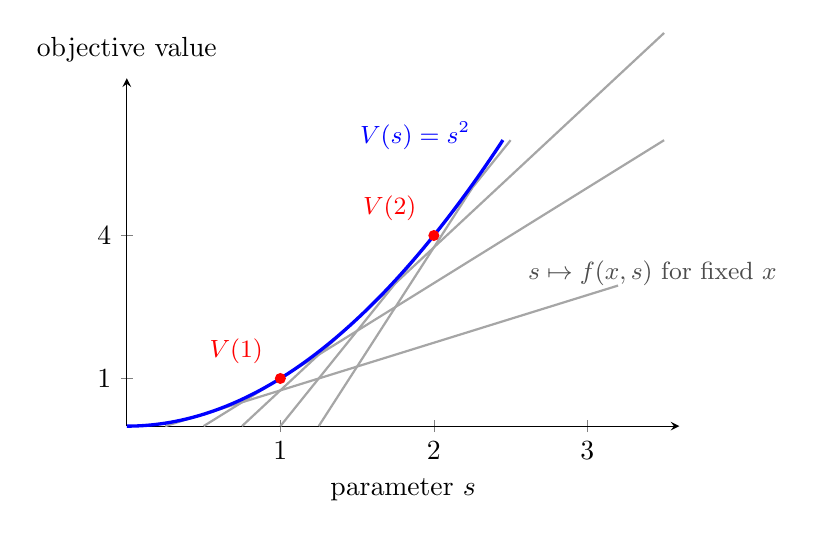
\begin{tikzpicture}
	\begin{axis}[
		axis lines=left, xmin=0, xmax=3.6, ymin=0, ymax=7.3,
		xtick={1,2,3}, ytick={1,4},
		xlabel={parameter $s$}, ylabel={objective value}, ylabel style={rotate=-90, anchor=south, at={(axis description cs:0,1.02)}},
		samples=80, smooth, width=8.6cm, height=6cm, clip=false
		]
		\addplot[gray!70, thick, domain=0.25:3.2, samples=2] {2*0.5*x-0.25};
		\addplot[gray!70, thick, domain=0.5:3.5, samples=2] {2*1*x-1};
		\addplot[gray!70, thick, domain=0.75:3.5, samples=2] {2*1.5*x-2.25};
		\addplot[gray!70, thick, domain=1.0:2.5, samples=2] {2*2*x-4};
		\addplot[gray!70, thick, domain=1.25:2.25, samples=2] {2*2.5*x-6.25};
		\addplot[blue, very thick, domain=0:2.45] {x^2};
		\fill[red] (axis cs:1,1) circle (2pt);
		\fill[red] (axis cs:2,4) circle (2pt);
		\node[red, anchor=south east, font=\small] at (axis cs:0.95,1.1) {$V(1)$};
		\node[red, anchor=south east, font=\small] at (axis cs:1.95,4.1) {$V(2)$};
		\node[blue, anchor=south east, font=\small] at (axis cs:2.3,5.6) {$V(s)=s^2$};
		\node[gray!60!black, anchor=west, font=\small] at (axis cs:2.55,3.2) {$s\mapsto f(x,s)$ for fixed $x$};
	\end{axis}
\end{tikzpicture}
\end{document}
